\documentclass[paper=a4,fontsize=12pt,ngerman]{scrartcl}

\usepackage[utf8]{inputenc}				
\usepackage[T1]{fontenc}
\usepackage{graphicx}
\usepackage[ngerman]{babel}
\usepackage{amsmath}
\usepackage[a4paper,left=25mm,right=35mm,top=25mm,bottom=30mm]{geometry}
\usepackage{parskip}
	

\begin{document}

\pagenumbering{roman}
\pagestyle{plain}

% Einbinden der Titelseite
\begin{titlepage}

\linespread{1.5}


\includegraphics[width=\linewidth]{graphics/htw_logo}

\begin{center}
    \large  
    \hfill
    \vfill
    \Large{\bfseries{Netzwerkstaukontrolle und die Arbeitsweise verschiedener Algorithmen in TCP}}\\
    
    von \\
    Michał Roziel

    Matrikelnummer : 5012845

    \vfill
		
    Ein wissenschaftlicher Bericht im Rahmen der Vorlesung\\
    \glqq Wissenschaftliches Arbeiten\grqq\\
    an der htw saar im Studiengang Informatik\\
	
    \vfill	
    \vfill
	
    Saarbrücken, den 30. August 2025
\end{center}
    
\end{titlepage}


% Hier ist der Abstract
\section*{Abstract}


\;
Im Rahmen dieses Berichts werden verschiedene Algorithmen Netzwerkstaukontrolle
In dem heutigen Stand von Computernetzwerken werden verschiedene Protokolle zur Netzwerkstaukontrolle genutzt, 
Ich werde mich im Rahmen dieses Berichts allerdings auf das Transmission Control Protocoll 
(Deutsch : \textit{Übertragungssteuerungsprotokoll, TCP}) beschränken, da dies das am meisten verbreitete ist.  
Die Algorithmen der Staukontrolle, welche in diesen Bericht einfließen sind : TCP Reno, TCP CUBIC, TCP ECN, und BBR.
\newline
Mittels des Netzwerk Emulators \textit{MiniNet} wird ein virtuelles Netzwerk zwischen zwei Endpunkten aufgestellt, über
welches ein Künstlicher Datenverkehr erzeugt wird.
Der genannte Datenverkehr wird anschließend aufgezeichnet und dient somit als Basis für den Vergleich der Staukontrolle durch 
die verschiedenen Algorithmen.
Die Auswertung, welche aus den Aufzeichungen stammt, ermöglicht dem Leser ein tieferes Verständnis über Staukontrolle in Computernetzwerken
zu erhalten. 





\newpage
\section*{Selbstständigkeitserklärung}
Ich versichere, dass ich die vorliegende Arbeit selbstständig verfasst und 
keine anderen als die angegebenen Quellen und Hilfsmittel benutzt habe.
Insbesondere habe ich alle KI-basierten Werkzeuge angegeben, die ich bei
der Erstellung, Übersetzung oder Überarbeitung des Textes verwendet habe.

Ich erkläre hiermit weiterhin, dass die vorgelegte Arbeit zuvor weder von mir 
noch von einer anderen Person an dieser oder einer anderen Hochschule 
eingereicht wurde.

Darüber hinaus ist mir bekannt, dass die Unrichtigkeit dieser Erklärung eine 
Benotung der Arbeit mit der Note \glqq nicht ausreichend\grqq \ zur Folge hat 
und einen Ausschluss von der Erbringung weiterer Prüfungsleistungen zur Folge 
haben kann.
\bigskip
 
Saarbrücken, den \today

\smallskip
Unterschrift  Michal Roziel




% Das Inhaltsverzeichnis
\clearpage
\tableofcontents 

\clearpage
\pagenumbering{arabic}

% Hier beginnt das erste Kapitel


\section{Einleitung}

Netzwerkstaukontrolle (Englisch : \textit{ Network congestion control, CC }) ist ein essentieller Bestandteil der 
meisten modernen Computernetzwerke. CC lässt sich in zu der Schicht 3 (Transportschicht) in dem OSI-Modell einordnen. 
Wenn eine Netzwerkschnittstelle zu einem Zeitpunkt versucht eine zu große Menge an Datenpaketen aufzunehmen,
kommt es zu Stau von Datenverkehr und zu einem potentiellen Verlust von Datenpaketen.
Aufgrund diesem Vorkommen werden Algorithmen innerhalb von Netzwerkprotokollen verwendet, diese erkennen den Anstau von Datenverkehr im Netzwerk,
und helfen den Fluss von Datenpaketen zu steuern. Neben dem effizienten Durchfluss von Informationen ist zeitgleich auch die ...



\subsection{Grundlagen und Begriffe}
In enim justo, rhoncus ut, imperdiet a, venenatis vitae, justo. Nullam dictum 
felis eu pede mollis pretium. Integer tincidunt. Cras dapibus. Vivamus 
elementum semper nisi.
\begin{figure}[h]
\begin{center}
  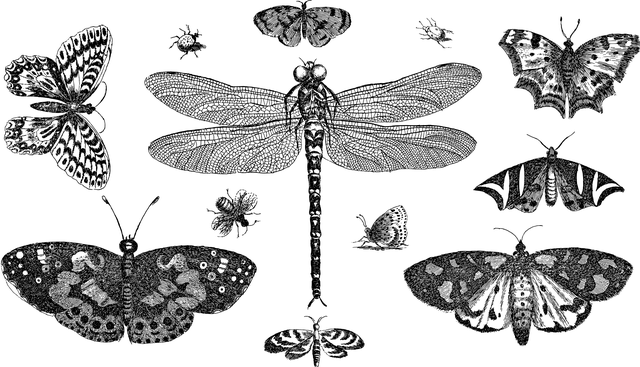
\includegraphics[scale=0.35]{graphics/insects-5304085_640.png}
  \caption{Schmetterlinge}
  \label{schmetter}
\end{center}
\end{figure}
Aenean vulputate eleifend tellus. Aenean leo ligula, porttitor eu, consequat 
vitae, eleifend ac, enim. Aliquam lorem ante, dapibus in, viverra quis, 
feugiat a, tellus. Lorem ipsum dolor sit amet, consectetuer adipiscing elit. 
Aenean commodo ligula eget dolor. Aenean massa. Cum sociis natoque penatibus 
et magnis dis parturient montes, nascetur ridiculus mus. Lorem ipsum dolor 
sit amet, consectetuer adipiscing elit. Aenean commodo ligula eget dolor. 
Aenean massa. Cum sociis natoque penatibus et magnis dis parturient montes, 
nascetur ridiculus mus.

\subsection{Definitionen}
Auch gibt es niemanden, der den Schmerz an sich liebt, sucht oder wünscht, 
nur, weil er Schmerz ist, es sei denn, es kommt zu zufälligen Umständen, in 
denen Mühen und Schmerz ihm große Freude bereiten können. Um ein triviales 
Beispiel zu nehmen, wer von uns unterzieht sich je anstrengender körperlicher 
Betätigung, außer um Vorteile daraus zu ziehen?

Aber wer hat irgend ein Recht, einen Menschen zu tadeln, der die Entscheidung 
trifft, eine Freude zu genießen, die keine unangenehmen Folgen hat, oder 
einen, der Schmerz vermeidet, welcher keine daraus resultierende Freude nach 
sich zieht? Auch gibt es niemanden, der den Schmerz an sich liebt, sucht oder 
wünscht, nur, weil er Schmerz ist, es sei denn, es kommt zu zufälligen 
Umständen, in denen Mühen und Schmerz ihm große Freude bereiten können. Um 
ein triviales Beispiel zu nehmen, wer von uns unterzieht sich je 
anstrengender körperlicher Betätigung, außer um Vorteile daraus zu ziehen? 
Aber wer hat irgend ein Recht, einen Menschen zu tadeln, der die Entscheidung 
trifft, eine Freude zu genießen, die keine unangenehmen Folgen hat, oder 
einen, der Schmerz vermeidet, welcher keine daraus resultierende Freude nach 
sich zieht? Auch gibt es niemanden, der den Schmerz an sich liebt.

\section{Analyse und Bewertung}
Phasellus viverra nulla ut metus varius laoreet. Quisque rutrum. Aenean 
imperdiet. Etiam ultricies nisi vel augue \cite{ab94}. Curabitur ullamcorper 
ultricies nisi. Nam eget dui. 
\begin{equation}
  \sum_{n=0}^N g_n(x) = \sum\nolimits_{n=0}^N g_n(x) =
  \int_a^b f(x) \,\mbox{d}x = \int\limits_a^b f(x) \,\mbox{d}x 
\end{equation}
Etiam rhoncus. Maecenas tempus, tellus eget condimentum rhoncus, sem quam 
semper libero, sit amet adipiscing sem neque sed ipsum. Nam quam nunc, 
blandit vel, luctus pulvinar, hendrerit id, lorem. Maecenas nec odio et ante 
\cite{ah2006} tincidunt tempus. Donec vitae sapien ut libero venenatis 
faucibus. Nullam quis ante. Etiam sit amet orci eget eros faucibus tincidunt. 
Duis leo. Sed fringilla mauris sit amet nibh. Donec sodales sagittis magna. 
Sed consequat, leo eget bibendum sodales, augue velit cursus nunc, quis 
gravida magna mi a libero. Fusce vulputate eleifend sapien.

\subsection{Die Verwandlung}
\glqq Jemand musste Josef K. verleumdet haben, denn ohne dass er etwas Böses 
getan hätte, wurde er eines Morgens verhaftet. Wie ein Hund! sagte er, es 
war, als sollte die Scham ihn überleben. Als Gregor Samsa eines Morgens aus 
unruhigen Träumen erwachte, fand er sich in seinem Bett zu einem ungeheueren 
Ungeziefer verwandelt. Und es war ihnen wie eine Bestätigung ihrer neuen 
Träume und guten Absichten, als am Ziele ihrer Fahrt die Tochter als erste 
sich erhob und ihren jungen Körper dehnte. Es ist ein eigentümlicher Apparat, 
sagte der Offizier zu dem Forschungsreisenden und überblickte mit einem 
gewissermaßen bewundernden Blick den Rest.\grqq \ (aus: \cite{kaf12})

\section{Ergebnisse und Diskussion}
Vestibulum purus quam, scelerisque ut, mollis sed, nonummy id, metus. Nullam 
accumsan lorem in dui. Cras ultricies mi eu turpis hendrerit fringilla. 
Vestibulum ante ipsum primis in faucibus orci luctus et ultrices posuere 
cubilia Curae; In ac dui quis mi consectetuer lacinia. Nam pretium turpis et 
arcu. Duis arcu tortor, suscipit eget, imperdiet nec, imperdiet iaculis, 
ipsum. Sed aliquam ultrices mauris. Integer \cite{m85} ante arcu, accumsana, 
consectetuer eget, posuere ut, mauris. Praesent adipiscing. Phasellus 
ullamcorper ipsum rutrum nunc. Nunc nonummy metus. Vestibulum volutpat 
pretium libero. Cras id dui. Aenean ut eros et nisl sagittis vestibulum. 
Nullam nulla eros, ultricies sit amet, nonummy id, imperdiet feugiat, pede.

\section{Fazit und Schlussfolgerungen}
Sed lectus. Donec mollis hendrerit risus. Phasellus nec sem in justo 
pellentesque facilisis. Etiam imperdiet imperdiet orci. Nunc nec neque. 
Phasellus leo dolor, tempus non, auctor et, hendrerit quis, nisi. Curabitur 
ligula sapien, tincidunt non, euismod vitae \cite{arrow48}, posuere 
imperdiet, leo. Maecenas malesuada. Praesent congue erat at massa. Sed cursus 
turpis vitae tortor. Donec posuere vulputate arcu. Phasellus accumsan cursus 
velit. Vestibulum ante ipsum primis in faucibus orci luctus et ultrices 
posuere cubilia Curae; 
\begin{table}[h]
\begin{center}
  \begin{tabular}{ |c|c|c| } 
    \hline
    Primzahlen & Tiere & Werkzeuge \\ 
    \hline
    17 & Elefant    & Schraubenzieher \\ 
    23 & Stechmücke & Zange \\ 
    \hline
  \end{tabular}
    \caption{Beispiel}
\end{center}
\end{table}
Sed aliquam, nisi quis porttitor congue, elit erat euismod orci, ac placerat 
dolor lectus quis orci. Phasellus consectetuer vestibulum elit. Aenean tellus 
metus, bibendum sed, posuere ac, mattis non, nunc. Vestibulum fringilla pede 
sit amet augue. In turpis. Pellentesque posuere. Praesent turpis. Aenean 
posuere, tortor sed cursus feugiat, nunc augue blandit nunc, eu sollicitudin 
urna dolor sagittis lacus (siehe Abbildung \ref{schmetter}). Donec elit 
libero, sodales nec, volutpat a, suscipit non, turpis. Nullam sagittis. 
Suspendisse pulvinar, augue ac venenatis condimentum, sem libero volutpat 
nibh, nec pellentesque velit pede quis nunc. Vestibulum ante ipsum primis in 
faucibus orci luctus et ultrices posuere cubilia Curae; Fusce id purus. Ut 
varius tincidunt libero. Phasellus dolor. Maecenas vestibulum mollis

\subsection{Offene Fragen}
Li Europan lingues es membres del sam familie. Lor separat existentie es un 
myth. Por scientie, musica, sport etc, litot Europa usa li sam vocabular. Li 
lingues differe solmen in li grammatica, li pronunciation e li plu commun 
vocabules. Omnicos directe al desirabilite de un nov lingua franca: On refusa 
continuar payar custosi traductores.

At solmen va esser necessi far uniform grammatica, pronunciation e plu sommun 
paroles. Ma quande lingues coalesce, li grammatica del resultant lingue es 
plu simplic e regulari quam ti del coalescent lingues. Li nov lingua franca 
va esser plu simplic e regulari quam li existent Europan lingues. It va esser 
tam simplic quam Occidental in fact, it va esser Occidental. A un Angleso it 
va semblar un simplificat Angles, quam un skeptic Cambridge amico dit me que 
Occidental es. Li Europan lingues es membres del sam familie. Lor separat 
existentie es un myth. Por scientie, musica,

\subsection{Diskussion}
Lorem ipsum dolor sit amet, consectetuer adipiscing elit. Aenean commodo 
ligula eget dolor. Aenean massa. Cum sociis natoque penatibus et magnis dis 
parturient montes, nascetur ridiculus mus. Donec quam felis, ultricies nec, 
pellentesque eu, pretium quis, sem. Nulla consequat massa quis enim. Donec 
pede justo, fringilla vel, aliquet nec, vulputate eget, arcu.

In enim justo, rhoncus ut, imperdiet a, venenatis vitae, justo. Nullam dictum 
felis eu pede mollis pretium. Integer tincidunt. Cras dapibus. Vivamus 
elementum semper nisi. Aenean vulputate eleifend tellus. Aenean leo ligula, 
porttitor eu, consequat vitae, eleifend ac, enim. Aliquam lorem ante, dapibus 
in, viverra quis, feugiat a, tellus. Phasellus viverra nulla ut metus varius 
laoreet. Quisque rutrum. Aenean imperdiet. Etiam ultricies nisi vel augue. 
Curabitur ullamcorper ultricies nisi. Nam eget dui. Etiam rhoncus. Maecenas 
tempus, tellus eget condimentum rhoncus, sem quam semper libero, sit amet 
adipiscing sem neque sed ipsum. Nam quam nunc, blandit vel, luctus pulvinar.

% Hier beginnt das Literaturverzeichnis
\clearpage
\renewcommand\refname{Literaturverzeichnis}
\bibliographystyle{alpha}
\bibliography{literatur}
\addcontentsline{toc}{section}{Literaturverzeichnis}


% Hier beginnt der Anhang
\clearpage
\appendix
\part*{Anhang}
\addcontentsline{toc}{section}{Anhang}

\section{Datenmaterial}
Li Europan lingues es membres del sam familie. Lor separat existentie es un 
myth. Por scientie, musica, sport etc, litot Europa usa li sam vocabular. Li 
lingues differe solmen in li grammatica, li pronunciation e li plu commun 
vocabules.

\section{Web-Standards}
Omnicos directe al desirabilite de un nov lingua franca: On refusa continuar 
payar custosi traductores. At solmen va esser necessi far uniform grammatica, 
pronunciation e plu sommun paroles. Ma quande lingues coalesce, li grammatica 
del resultant lingue es plu simplic e regulari quam ti del coalescent 
lingues. Li nov lingua franca va esser plu simplic e regulari quam li 
existent Europan

\end{document}

